\documentclass{midl} % Include author names

% The following packages will be automatically loaded:
% jmlr, amsmath, amssymb, natbib, graphicx, url, algorithm2e
% ifoddpage, relsize and probably more

\jmlrvolume{-- Under Review}
\jmlryear{2027}
\jmlrworkshop{Full Paper -- MIDL 2027 submission}
\editors{Under Review for MIDL 2027}

\title[Short Title]{Full Title of Article}

% Single-blind: author names are revealed at submission.
% NOTE: the author list is FINAL at submission time -- no additions,
% removals or reordering after the deadline.
\midlauthor{\Name{Jungro Lee\nametag{$^{1}$}} \Email{firstauthor@ucl.ac.uk}\\
\Name{Petru Manescu\nametag{$^{1}$}} \Email{p.manescu@ucl.ac.uk}\\
\addr $^{1}$ Department of Computer Science, University College London, London, UK
}

\begin{document}

\maketitle

\begin{abstract}
% Abstract registration deadline: 2026-11-30 AoE.
\end{abstract}

\begin{keywords}
% comma separated
\end{keywords}

% =====================================================================
% Page budget (main text limit: 10 pages, excluding references,
% acknowledgements and appendix).
%   Introduction ............ 1.5 p
%   Related Work ............ 0.5 p
%   Methods ................. 2.0 p
%   Experiments and Results . 4.0 p
%   Discussion .............. 1.0 p
%   Conclusion .............. 0.3 p
% Reviewers are not obliged to read the appendix: anything that
% determines the evaluation must sit inside the 10 main pages.
% =====================================================================

\section{Introduction}
\label{sec:introduction}

Most breast cancers are found at an early stage, they are also hormone receptor-positive and
human epidermal growth factor receptor 2-negative (HR+/HER2$-$). These patients have surgery
and then endocrine therapy. The remaining question is whether to add chemotherapy. Only a
minority of them benefit from it, and the rest take on its side effects for nothing. Multi-gene
assays were therefore built to estimate the risk of recurrence from tumour gene expression. The
most widely used one is the 21-gene recurrence score (RS) \citep{paik2004, sparano2018}. The
assay works, but it is costly, which takes several thousand pounds per patient. It consumes
tumour tissue, of which result also arrives one to two weeks after a pathologist has already read
the haematoxylin and eosin (H\&E) slide. A model that predicts the RS from that slide would
not replace the assay, but it could instead triage which patients are sent for genomic testing,
and it would cost no extra tissue and no extra waiting. This is possible because two gene
groups dominate the score, namely proliferation and oestrogen signalling, which leave visible
traces in nuclear shape and in tissue architecture \citep{paik2004, elston1991}. These molecular
readouts have already been recovered from H\&E before. Examples include driver mutations
\citep{coudray2018}, microsatellite instability \citep{kather2019} and bulk expression
\citep{schmauch2020}. For the RS itself, hand crafted nuclear shape features
\citep{whitney2018} and deep learning \citep{howard2024} have both been tried.

Predicting tasks from a whole-slide image (WSI) runs first into size. A slide scanned at
$40\times$ spans on the order of $10^5 \times 10^5$ pixels and it also carries a single label,
and that label belongs to no particular region. Multiple instance learning (MIL) is the
standard answer to this. First, the slide becomes a bag of patches and each patch is encoded on its own.
A permutation invariant pooling function then turns the bag into one slide representation
\citep{dietterich1997, ilse2018, campanella2019}. The patch encoder has improved steadily
inside this formulation. It moved from ImageNet-pretrained convolutional networks
\citep{he2016, lu2021} to self-supervised pathology encoders, and then to foundation models
trained on $10^5$--$10^6$ slides \citep{chen2024, filiot2023}. The patch budget has not had
the same attention. Some pipelines tile the tissue exhaustively \citep{campanella2019, lu2021}.
Others sample $10^3$--$10^4$ tiles per slide \citep{courtiol2018, wulczyn2020}. 

A second limit is representation of molecular functions within the image. Pooling over patch embeddings throws away where the
patches were. Therefore, a patch embedding also describes local texture rather than the individual cells
and how they relate \citep{ilse2018, pati2022}. Graph neural networks (GNNs) were brought into
computational pathology to put this structure back. They are used at two granularities. In the
first, patches are the nodes and spatial adjacency gives the edges, as in SlideGraph+
\citep{lu2022} and Patch-GCN \citep{chen2021}. Second, each segmented nucleus become a
node and it carries a morphometric descriptor, which is joined to the nuclei near it
\citep{zhou2019, pati2022}. The model then reads tissue architecture directly instead of
inferring it from texture. A pathologist grades nuclear size, chromatin
density, crowding and tubule formation, and in a cell graph these are explicit properties
rather than latent directions in an embedding.

We combine the two views, and we ask how much tissue a model actually needs to see. Each slide
is reduced to a small number of pathches $N$ of tissue regions of $1 \times 1$\,mm ($4096$ pixels at
$0.25\,\mu$m/px). HoVer-Net \citep{graham2019} segments the nuclei inside a region. Those
nuclei form one cell graph that spans the whole region, with morphometric descriptors as node
features. The region is also split into sixteen tiles, and a frozen UNI2-h encoder embeds
each one. A learned gate fuses the graph embedding with those tile embeddings, and the region
vectors are then aggregated to the slide. We hold the architecture fixed and vary $N$ from 2
to 16. We evaluate on The Cancer Genome Atlas (TCGA) and on two external cohorts. RS prediction
saturates at small area, which is about $4\,\mathrm{mm}^2$ of tissue per slide, far below the
budgets used in the literature. From this, we found that the signal that matters for the RS is therefore not limited by
spatial coverage. It is no longer how much of the slide to
process, but which morphological properties carry the signal. Therefore, we address the second question
by relating graph morphology and cell-type composition to receptor status and to the
recurrence score.

Our contributions are as follows.
\begin{itemize}
\item A region level dual branch model is designed with gated module to reflect both morphological features' relation and spatial feature of the image. 
\item A controlled study of the region budget, with $N \in \{2,4,8,16\}$ nested regions per
  slide was conducted. 
\item An analysis of which graph morphology features and cell types are associated with
  HER2/PR status and with the recurrence score was conducted to identify where the predictive signal
  resides, not only how much tissue is needed to find it.
\end{itemize}
\section{Related Work}
\label{sec:related-work}

\paragraph{Nuclear segmentation: HoVer-Net.}
HoVer-Net \citep{graham2019} describes individual nuclei in histopathology image. It is consisted of a single encoder with three
decoder branches. One branch segments nuclear pixels, and a second regresses the horizontal and
vertical distances from each pixel to the centre of mass of its nucleus, which lets
the model split nuclei that touch. Lastly, a third assigns each instance a type. We use the weights
trained on PanNuke \citep{gamper2020}, a dataset of 205,343 labelled nuclei drawn from 19
tissue types and annotated into five classes: neoplastic, non-neoplastic epithelial,
inflammatory, connective or soft tissue, and dead. For comparison, the dataset used in the
original HoVer-Net paper held roughly 24,000 labelled nuclei from a single tissue type, so the
PanNuke weights transfer far better across organs. The output per nucleus is a contour, a
centroid, a class and a confidence.  Cell graphs in pathology are commonly built on them, as in CGC-Net \citep{zhou2019} and
HACT-Net \citep{pati2022}.

\paragraph{Patch encoding: UNI2-h.}
UNI \citep{chen2024} describes whole patches instead of single cells. It is a vision
transformer trained with DINOv2 \citep{oquab2024}, so no labels are used. The model learns
tissue features in two ways. It matches different views of the same image, and it fills in
masked regions from their surroundings. UNI2-h, the variant we use, is a ViT-H/14 of roughly
681M parameters. It was trained on more than 200 million patches from over 350,000 slides. Its
pretraining is documented not to include TCGA, which keeps our TCGA evaluation uncontaminated.
In an independent benchmark it ranked near the top across slide and patch level tasks
\citep{campanella2025}. The output is one embedding vector per patch. Such frozen embeddings
now serve as the instance features in most MIL pipelines \citep{lu2021, filiot2023}. 

\paragraph{Super-resolution: Swin2SR.}
Our cohorts are not scanned at the same magnification, and HoVer-Net is sensitive to this.
Nuclei that touch cannot be separated when they occupy too few pixels, which force us to upsample
the lower-magnification cohort before segmentation, using Swin2SR \citep{conde2022}. Swin2SR
is a transformer built on Swin V2 blocks \citep{liu2022}. It computes self-attention inside
local windows, and it shifts those windows between consecutive layers. This captures context
across windows while keeping the cost linear in the number of pixels. The $\times 4$ variant
we use is trained on DF2K, a collection of natural images, with bicubically downsampled inputs
and an $\ell_1$ pixel loss. However, it is therefore a general-purpose model and has seen no
histopathology. That turns out to be acceptable in this paper, \citet{juhong2023} report that
transformer-based super-resolution transfers to H\&E without retraining, at only a modest
cost in downstream segmentation. 

\paragraph{Message passing over cell graphs.}
A GNN updates each node from its neighbours, so the three operators we compare differ only in
how a node weights them. We write $h^{(l)}_i$ for the embedding of node $i$ at layer $l$ and
$\mathcal{N}(i)$ for its neighbourhood. GCN \citep{kipf2017} applies a symmetric normalised
convolution,
\begin{equation}
\label{eq:gcn}
h^{(l+1)}_{i} = \sigma\!\left( \sum_{j \in \mathcal{N}(i) \cup \{i\}}
\frac{W^{(l)} h^{(l)}_{j}}{\sqrt{\hat{d}_i \hat{d}_j}} \right),
\end{equation}
where $\hat{d}_i$ is the degree of node $i$ including its self-loop. The normalising term
damps the degree signal without removing it. GraphSAGE \citep{hamilton2017} averages the
neighbours and combines that average with the node's own state through separate weights,
\begin{equation}
\label{eq:sage}
h^{(l+1)}_{i} = \sigma\!\left( W^{(l)}_{1} h^{(l)}_{i} + W^{(l)}_{2} \cdot
\frac{1}{|\mathcal{N}(i)|} \sum_{j \in \mathcal{N}(i)} h^{(l)}_{j} \right).
\end{equation}
The mean removes degree entirely, so crowding can reach the representation only through which
nodes are reachable. GIN \citep{xu2019} sums over the neighbours and then applies an MLP,
\begin{equation}
\label{eq:gin}
h^{(l+1)}_{i} = \mathrm{MLP}^{(l)}\!\left( \left(1 + \epsilon^{(l)}\right) h^{(l)}_{i}
+ \sum_{j \in \mathcal{N}(i)} h^{(l)}_{j} \right).
\end{equation}
GIN is the only one of the three whose aggregation is not degree-normalised. The sum grows
with the number of neighbours, so local density enters the representation directly. 

\paragraph{Edge derivation in cell graphs.}
The edge rule decides which notion of neighbourhood the
graph encodes. Among various ways, delaunay triangulation joins nuclei whose Voronoi cells share a boundary. The
result is a connected planar graph that approximates physical cell contact. It is the usual
choice when the graph should represent tissue architecture rather than mere proximity
\citep{gunduz2004, lu2022}. In this paper, its decisive property is that it needs no scale parameter.
We also tested with other methods, A radius rule instead ties connectivity to a distance, and that distance is tuned to one
cohort's nuclear spacing \citep{pati2022}. A $k$-nearest-neighbour rule fixes $k$ in advance
\citep{zhou2019}. 

\paragraph{Predicting the recurrence score from H\&E.}
The 21-gene recurrence score summarises the expression of sixteen cancer-related genes. These
are normalised against five reference genes and aggregated into four functional group scores
\citep{paik2004}. The unscaled score is a fixed weighted sum of those groups,
\begin{equation}
\label{eq:rs}
\begin{split}
\mathrm{RS}_{u} = \;&+0.47\,\mathrm{HER2} - 0.34\,\mathrm{ER} + 1.04\,\mathrm{Prolif}
+ 0.10\,\mathrm{Invasion} \\
&+ 0.05\,\mathrm{CD68} - 0.08\,\mathrm{GSTM1} - 0.07\,\mathrm{BAG1},
\end{split}
\end{equation}
where each term is the expression score of a gene group (ER: oestrogen receptor group; Prolif:
proliferation group) or of a single gene. The HER2 and proliferation group scores are
thresholded from below before they enter \equationref{eq:rs}. The result is then rescaled to
the reported $0$--$100$ range as
$\mathrm{RS} = \min\{100, \max\{0,\, 20(\mathrm{RS}_{u} - 6.7)\}\}$ \citep{paik2004}. In this equation, the proliferation group carries the largest positive weight, and the
oestrogen group carries the only substantial negative one. This is what makes the score
accessible from morphology at all. Proliferation is visible as enlarged nuclei, dense
chromatin, mitotic figures and crowding. Oestrogen signalling instead accompanies a
differentiated, tubule-forming architecture with uniform nuclei \citep{elston1991}.  Thanks to these properties, molecular
readouts have accordingly been recovered from H\&E in several settings. Two previous studies address the recurrence score directly.
\citet{whitney2018} showed that hand-crafted nuclear shape features separate low- from
high-risk categories. \citet{howard2024} reported an area under the receiver operating
characteristic curve (AUROC) of 0.797 on the TCGA breast cancer cohort (TCGA-BRCA) with
patch-based deep learning. 

\section{Methods}
\label{sec:methods}

% Figure: Dissertation/code/figures/latex/fig_pipeline_regions_server.py
\begin{figure}[htbp]
\floatconts
  {fig:pipeline}
  {\caption{Pipeline on one TCGA slide. (a)--(c) Tissue detection and the sixteen nested
  regions, coloured by the smallest budget $N$ that includes them. (d) One $4096$-pixel region
  with the $4 \times 4$ grid of tiles embedded by UNI2-h (box: zoom of (e)). (e) HoVer-Net
  nuclei coloured by type (red neoplastic, blue inflammatory, green connective, orange
  non-neoplastic epithelial). (f) The Delaunay cell graph spanning the whole region across tile
  boundaries (dashed). Bottom: the dual-branch model.}}
  {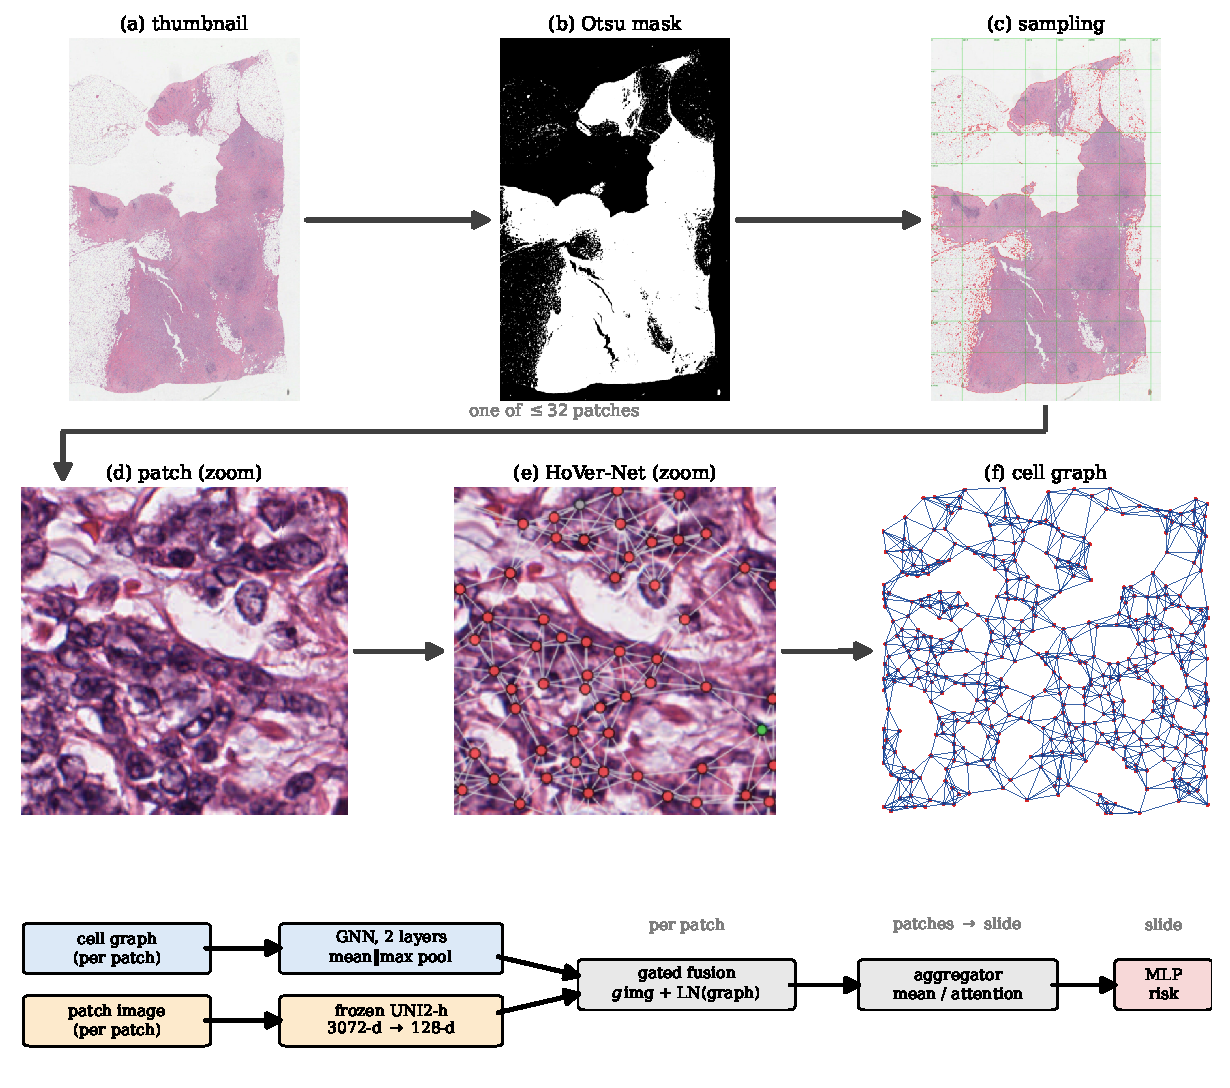
\includegraphics[width=0.8\linewidth]{figures/fig_pipeline.pdf}}
\end{figure}

\figureref{fig:pipeline} summarises the pipeline. A slide is reduced to $N$ tissue regions of
$4096 \times 4096$ pixels at $0.25\,\mu$m/px; each region yields one cell graph and sixteen
tile embeddings, the two are fused per region, and the regions are aggregated to the slide.

\subsection{Region-Level Cell Graph Construction}
\label{sec:cell-graph-construction}

\paragraph{Regions.}
Tissue is separated from background glass by Otsu thresholding of a low-resolution level of
the slide. Candidate windows of $4096 \times 4096$ level-0 pixels ($1.02$\,mm on a side) are
laid on a half-window stride, windows with a tissue fraction below 0.6 are discarded (0.3 if
none survive), and $N$ non-overlapping windows are drawn at random with a seed fixed per
slide. A region is the unit seen by both branches: it is large enough to contain glandular
and stromal architecture, yet small enough for a single cell graph to cover it.

\paragraph{Resolution harmonisation.}
The three cohorts are scanned at different magnifications, and nuclear segmentation is the
step that is sensitive to this difference: a model trained to delineate nuclei at $40\times$
under-segments lower-magnification input, since touching nuclei occupy too few pixels to be
separated. We therefore harmonise resolution before segmentation rather than after, with the
transformer-based super-resolution model Swin2SR \citep{conde2022}. Slides scanned at
$20\times$ (51 TCGA slides and 144 of the 273 CPTAC-BRCA series) are cut at 2048 pixels and
upsampled $\times 2$. The UCH cohort is distributed only as $299$-pixel tiles at
$1.01\,\mu$m/px ($\approx 10\times$); a region is formed from a $4 \times 4$ block of
adjacent tiles that all contain tissue, stitched to 1196 pixels, centre-cropped to 1024
pixels ($1.03$\,mm) and upsampled $\times 4$. Every region therefore enters segmentation with
the same physical field and the same effective $0.25\,\mu$m/px. To verify that $\times 4$
upsampling does not fabricate structure, we segment TCGA fields for which both a native
$40\times$ scan and a super-resolved $10\times$ version exist and match detections by centroid
proximity: instance-level agreement reaches an F1 of 0.860 and cell-type accuracy 0.887. The
latter is the relevant quantity, since the node features and graph statistics depend on the
population of nuclei rather than on any individual detection.

\paragraph{Nuclear segmentation.}
Each region is passed whole through HoVer-Net \citep{graham2019} with PanNuke-pretrained
weights, in tile mode with overlapping stitching, so nuclei on internal tile boundaries are
not cut. HoVer-Net regresses horizontal and vertical distance maps alongside the nuclear
mask, which separates touching nuclei that a purely semantic model merges, and a
classification branch assigns each instance one of six PanNuke classes: neoplastic,
inflammatory, connective or soft tissue, necrotic, non-neoplastic epithelial, and an
unlabelled background class. For every nucleus we retain the centroid, the polygonal contour,
the axis-aligned bounding box, the predicted type and its confidence. A TCGA region contains
on average 3,971 nuclei (median 3,855, interquartile range 2,286--5,198), against 2,664 in UCH
and 4,122 in CPTAC-BRCA. Regions with too few nuclei to triangulate, which are background,
yield no graph and are discarded.

\paragraph{Node features.}
Each nucleus becomes a node with a $13$-dimensional morphometric descriptor built entirely from
the HoVer-Net output: the centroid (2), a one-hot encoding of the six PanNuke classes (6), the
type confidence (1), and four shape terms, namely log nuclear area, log perimeter,
bounding-box aspect ratio and convexity (4). Centroid and shape terms are $z$-scored within
the region. Every term corresponds to something a pathologist grades: nuclear enlargement and
pleomorphism are two of the three components of the Nottingham grade, aspect ratio separates
elongated stromal nuclei from rounder tumour nuclei, and convexity is low for the notched
nuclei of high-grade carcinoma.

\paragraph{Edges.}
Edges are derived from the centroid coordinates by Delaunay triangulation, which connects
nuclei whose Voronoi cells are adjacent. One graph spans the whole region, running straight
across the boundaries of the sixteen tiles seen by the image branch. The rule requires no
scale parameter, and its degree statistics are unchanged across cohorts whose nuclear density
is not: the mean degree is 5.97 in TCGA, UCH and CPTAC-BRCA alike, although a UCH region holds
a third fewer nuclei than a TCGA region of the same area.

\subsection{Dual-Branch Architecture}
\label{sec:dual-branch-architecture}

\paragraph{Graph branch.}
The region graph is processed by a graph convolutional network (GCN) \citep{kipf2017} of
$L=3$ layers and width $d_g=128$, each layer followed by batch normalisation, ReLU and dropout.
Node embeddings $h_i$ are pooled by concatenating their mean and element-wise maximum and
projecting back to $d_g$,
\begin{equation}
\label{eq:region-readout}
z^{g}_{r} = \mathrm{LayerNorm}\!\left( \mathrm{ReLU}\!\left( W \left[ \tfrac{1}{|V_r|}
\textstyle\sum_{i \in V_r} h_i \;\big\|\; \max_{i \in V_r} h_i \right] \right) \right),
\end{equation}
where $V_r$ is the node set of region $r$. The readout retains both the typical nucleus and
the most extreme one, since a single highly abnormal nucleus can be diagnostically decisive.

\paragraph{Image branch.}
The same region is divided into a $4 \times 4$ grid of 1024-pixel tiles. Because UNI2-h
\citep{chen2024} expects roughly 224-pixel inputs and downsampling a 1024-pixel tile that far
would blur away cell-level detail, each tile is further divided into a $4 \times 4$ grid of
256-pixel views, each view is resized and embedded by the frozen encoder (class token
concatenated with the mean patch token, 3072-d), and the sixteen view embeddings are averaged.
Each tile vector is projected to 128 dimensions by LayerNorm, a linear map, ReLU and dropout,
and the sixteen tiles are pooled by gated attention \citep{ilse2018} and normalised, giving
$z^{u}_{r}$. The encoder is frozen throughout: the question is what the graph adds on top of a
strong image representation, and that comparison is only clean if the image representation
cannot co-adapt to the graph branch.

\paragraph{Gated fusion.}
The two branches are combined at region level, before slide aggregation, by a single learned
scalar that scales the image branch against the normalised graph branch,
\begin{equation}
\label{eq:fusion}
z_{r} = \left[\, g \cdot z^{u}_{r} \;\big\|\; z^{g}_{r} \,\right],
\end{equation}
where $g$ is initialised at 1 and learned with the rest of the network. Because both branch
outputs are layer-normalised, $g$ is directly interpretable as the relative weight of the image
branch: $g>1$ means the image branch dominates, $g<1$ the cell graph, and we report it as a
result.

\paragraph{Region attention MIL.}
The fused region vectors $\{z_r\}_{r=1}^{N}$ of a slide are reduced to a single slide vector by
gated attention pooling \citep{ilse2018},
\begin{equation}
\label{eq:abmil}
z_{S} = \sum_{r} a_{r} z_{r}, \qquad
a_{r} = \frac{\exp\!\left( w^{\top} \left( \tanh(V z_{r}) \odot \sigma(U z_{r}) \right) \right)}
{\sum_{q} \exp\!\left( w^{\top} \left( \tanh(V z_{q}) \odot \sigma(U z_{q}) \right) \right)},
\end{equation}
where $\sigma$ is the logistic sigmoid, so that the weights $a_r$ can be read directly as
region importance and inspected against the morphology of the regions they select.

\paragraph{Prediction head and loss.}
The slide vector passes through LayerNorm, a linear layer of width 64, ReLU and dropout into a
single logit. One model is trained per target (binarised RS, PR status, HER2 status) with a
class-weighted binary cross-entropy,
\begin{equation}
\label{eq:loss}
\mathcal{L} = -\frac{1}{|B|} \sum_{S \in B} \Big[ \omega\, y_S \log \hat{p}_S
+ (1 - y_S) \log (1 - \hat{p}_S) \Big], \qquad \omega = \frac{n_{-}}{n_{+}},
\end{equation}
where $n_{+}$ and $n_{-}$ count the positive and negative training slides. Predicting the
receptor states with the same architecture is not an auxiliary exercise. The recurrence score
is itself a weighted combination of a HER2 group and an oestrogen group
(\equationref{eq:rs}), so a model that recovers the receptor states from morphology is
recovering the constituents of the quantity it is asked to predict, and the three targets give
three views of the same question of where the signal resides. Two ablations drop one branch
from \equationref{eq:fusion}: \emph{image-only} and \emph{graph-only}.

\subsection{Region Budget Protocol}
\label{sec:region-sampling-protocol}

The budget $N \in \{2, 4, 8, 16\}$ is the quantity we vary, which corresponds to roughly
2--16\,mm$^2$ of tissue per slide. $N=2$ matches the segmentation budget of a conventional
32-patch pipeline ($2 \times 16$ tiles of 1024 pixels). Region draws are nested: the windows are
taken by a greedy pass over the same seeded shuffle, so the first $k$ regions of a 16-region
draw are exactly the $k$-region draw, and every larger budget adds tissue to the smaller one
instead of replacing it. All other components are held fixed while $N$ is swept, so the
resulting curve isolates the dependence on coverage. Slides with little tissue contribute fewer
regions: at $N=16$ a TCGA slide holds 15.8 regions on average, and 1,047 of 1,096 slides reach
the full sixteen. All regions of a slide are used in training and inference.

\section{Experiments and Results}
\label{sec:experiments}

% ~4 pages total across the three subsections.

\subsection{Setup}
\label{sec:setup}

\paragraph{TCGA-BRCA (internal).}
Diagnostic formalin-fixed sections were streamed from the NCI Imaging Data Commons. 1,096
slides from 1,038 patients yield at least the first two regions; 51 slides scanned at
$20\times$ are harmonised as described in \sectionref{sec:cell-graph-construction}. Labels are
taken from the TCGA clinical fields used by \citet{guo2026}. TCGA never ran the commercial
Oncotype DX assay, so the RS label is a research-grade score computed from bulk RNA sequencing
of the 21 genes with \equationref{eq:rs} \citep{paik2004}, thresholded at the 85th percentile
of the HR+/HER2$-$ subset following \citet{howard2024}; this places 302 of the 1,038 patients
in the high-risk class. PR status is taken from immunohistochemistry (IHC; 986 patients, 661
positive) and HER2 status from the clinical HER2 call with equivocal cases removed (843
patients, 146 positive).

\paragraph{UCH (external).}
The external cohort was collected at the University of Chicago Hospital (UCH) and, unlike
TCGA, carries clinically assayed Oncotype DX scores, which makes it the stricter test of
generalisation: the model must transfer across scanner, magnification and label provenance.
Slides with $\mathrm{RS} \geq 26$ are labelled high risk, giving 417 patients (472 slides, 77
high risk). PR and HER2 status come from the clinical IHC record (PR: 500 patients, 439
positive; HER2: 487 patients, 9 positive). A UCH slide yields 14.6 regions on average at
$N=16$, fewer than a TCGA slide, because a region requires a complete $4 \times 4$ block of
tissue tiles.

\paragraph{CPTAC-BRCA (external).}
The second external cohort is the Clinical Proteomic Tumor Analysis Consortium breast cancer
cohort (CPTAC-BRCA), a mix of $40\times$ and $20\times$ scans that, like TCGA, has no clinical
assay. We compute a surrogate RS from RNA sequencing: $\log_2(\mathrm{TPM}+1)$ expression is
normalised to the five reference genes, each gene is min--max scaled to 0--15 across the
cohort, and \equationref{eq:rs} is applied. A patient is labelled high risk if
$\mathrm{RS}_u \geq 12.24$, a cut-off fixed before any model was applied, which places the same
fraction of the 122 CPTAC patients with slides in the high-risk class as in TCGA (28.7\%).
108 patients (263 slides, 34 high risk) yield regions; only the RS target is available.

\paragraph{Protocol.}
Internal evaluation follows the protocol of \citet{guo2026}: patient-level, label-stratified
five-fold cross-validation with a 7:1:2 train/validation/test ratio per fold. Their split
files are not released, so the splits are regenerated with the same protocol and a fixed seed,
and every model in this paper uses the same files. Every slide of a patient falls in the same
partition, and a patient's score is the mean of their slide probabilities. All patients are
evaluated, not only the HR+/HER2$-$ subset. We report the mean and standard deviation of the
test AUROC over the five folds. The external cohorts are never used for model selection: each
configuration is applied as the ensemble of its five fold models (mean of the five slide
probabilities) without retraining or recalibration, and we report patient-level AUROC with a
95\% confidence interval from 2,000 patient bootstrap resamples.

\paragraph{Random seeds.}
Three sources of randomness are fixed so that every comparison in this section is paired. The
region draw of each slide is seeded by the slide itself (the last eight digits of its Imaging
Data Commons series UID for TCGA, a CRC32 hash of the slide name for UCH and CPTAC), so every
model, every budget $N$ and every rerun sees exactly the same tissue, and the nested draws of
\sectionref{sec:region-sampling-protocol} follow from the same shuffle. The five splits are
generated once per target with seed 1 (validation patients of fold $f$ with seed $1+f$) and
shared by all models. Fold $f$ is trained with seed $42+f$ for weight initialisation, batch
order and dropout. The reported standard deviation is therefore the
spread across folds, i.e.\ across disjoint test patients, rather than across seeds.

\paragraph{Training.}
Models are trained for 60 epochs with AdamW (learning rate $10^{-4}$, weight decay $10^{-3}$)
and cosine annealing to $10^{-6}$, a batch of four slides and dropout 0.3, on a single
GPU. The checkpoint with the best patient-level validation AUROC is evaluated on the test fold.
Graphs and tile embeddings are pre-computed, so training cost is dominated by the GNN and grows
linearly with $N$.

% TODO: wall-clock / memory per N (inference cost) for contribution 2

\subsection{Does More Region Sampling Help?}
\label{sec:more-region-sampling}

\begin{table}[htbp]
\floatconts
  {tab:tcga}
  {\caption{Internal five-fold AUROC (\%, mean $\pm$ SD over folds) on TCGA-BRCA as the number
  of regions per slide $N$ grows. Image: image branch only; Graph: graph branch only; Gated:
  both, fused by \equationref{eq:fusion}.}}
  {\small
  \begin{tabular}{llcccc}
  \hline
  Target & Model & $N=2$ & $N=4$ & $N=8$ & $N=16$ \\
  \hline
  RS   & Image & 84.2 $\pm$ 4.0 & 86.1 $\pm$ 4.1 & 85.9 $\pm$ 3.8 & 86.1 $\pm$ 4.7 \\
       & Graph & 76.2 $\pm$ 3.5 & 78.7 $\pm$ 5.9 & 80.4 $\pm$ 3.2 & 79.7 $\pm$ 5.0 \\
       & Gated & 85.1 $\pm$ 3.9 & 85.9 $\pm$ 4.2 & 86.3 $\pm$ 4.0 & 85.5 $\pm$ 3.1 \\
  \hline
  PR   & Image & 76.8 $\pm$ 3.6 & 77.9 $\pm$ 1.6 & 78.9 $\pm$ 1.7 & 81.3 $\pm$ 2.6 \\
       & Graph & 65.5 $\pm$ 3.0 & 67.5 $\pm$ 2.5 & 70.6 $\pm$ 5.6 & 73.1 $\pm$ 4.0 \\
       & Gated & 76.8 $\pm$ 3.3 & 77.8 $\pm$ 2.3 & 79.3 $\pm$ 1.7 & 79.2 $\pm$ 2.1 \\
  \hline
  HER2 & Image & 69.9 $\pm$ 2.4 & 68.5 $\pm$ 4.5 & 72.3 $\pm$ 3.3 & 73.1 $\pm$ 2.6 \\
       & Graph & 62.1 $\pm$ 3.5 & 60.0 $\pm$ 5.8 & 63.3 $\pm$ 5.6 & 63.8 $\pm$ 5.7 \\
       & Gated & 70.3 $\pm$ 4.6 & 71.1 $\pm$ 3.5 & 73.0 $\pm$ 3.8 & 74.0 $\pm$ 2.4 \\
  \hline
  \end{tabular}}
\end{table}

\begin{table}[htbp]
\floatconts
  {tab:external}
  {\caption{External patient-level AUROC (\%) [95\% bootstrap CI] of the five-fold ensemble
  trained on TCGA, without retraining. CPTAC-BRCA has an RNA-derived RS only. UCH HER2 has nine
  positive patients and is reported for completeness.}}
  {\small
  \begin{tabular}{llcccc}
  \hline
  Cohort / target & Model & $N=2$ & $N=4$ & $N=8$ & $N=16$ \\
  \hline
  CPTAC RS   & Image & 78.0 [66, 88] & 81.3 [71, 90] & 81.2 [71, 90] & 81.9 [72, 90] \\
  (108 / 34) & Graph & 74.0 [64, 84] & 76.0 [65, 86] & 74.0 [63, 84] & 72.9 [62, 83] \\
             & Gated & 78.8 [69, 88] & 85.1 [76, 93] & 84.0 [74, 92] & 83.4 [74, 91] \\
  \hline
  UCH RS     & Image & 72.1 [65, 78] & 75.1 [68, 82] & 76.4 [70, 82] & 75.1 [69, 81] \\
  (417 / 77) & Graph & 62.7 [56, 69] & 64.6 [57, 72] & 66.6 [60, 73] & 68.6 [62, 75] \\
             & Gated & 72.7 [66, 79] & 74.3 [68, 80] & 75.5 [69, 82] & 75.2 [69, 81] \\
  \hline
  UCH PR      & Image & 67.3 [59, 75] & 67.0 [59, 75] & 67.2 [59, 75] & 66.6 [59, 74] \\
  (500 / 439) & Graph & 57.1 [50, 64] & 56.6 [49, 64] & 56.7 [49, 65] & 57.6 [50, 65] \\
              & Gated & 65.9 [58, 74] & 65.5 [57, 74] & 67.1 [59, 75] & 67.3 [60, 74] \\
  \hline
  UCH HER2    & Image & 57.1 [32, 80] & 59.9 [41, 79] & 59.6 [38, 81] & 64.6 [46, 83] \\
  (487 / 9)   & Graph & 41.4 [23, 59] & 42.9 [23, 62] & 52.3 [30, 73] & 56.0 [36, 74] \\
              & Gated & 57.7 [35, 78] & 54.9 [35, 75] & 54.9 [36, 75] & 59.2 [38, 81] \\
  \hline
  \end{tabular}}
\end{table}

\tableref{tab:tcga} reports internal performance. For the recurrence score the image-only and
gated models reach their plateau by $N=4$ (86.1 and 85.9) and gain nothing further at $N=8$ or
$N=16$; every change beyond $N=4$ is well inside one fold standard deviation. Receptor status
behaves differently: image-only PR rises monotonically from 76.8 at $N=2$ to 81.3 at $N=16$,
and gated HER2 from 70.3 to 74.0. The graph-only model benefits most from coverage (RS $+3.5$,
PR $+7.6$ points from $N=2$ to $N=16$) but remains 6--12 points below the image branch at every
budget. Gated fusion matches the image-only model within one standard deviation in every cell,
and the learned gate settles between $g=1.02$ and $g=1.10$ in all twelve gated configurations,
weighting the image branch only marginally above the cell graph.

\tableref{tab:external} shows that the saturation of the RS carries over to both external
cohorts. On CPTAC-BRCA the gated model rises from 78.8 at $N=2$ to 85.1 at $N=4$ and stays at
83--84 thereafter, exceeding the image-only model by 1.5--3.8 points at every $N \geq 4$; on
UCH, RS discrimination improves from 72.7 to 75.5 at $N=8$ and is flat at $N=16$, with
image-only and gated models indistinguishable. All confidence intervals overlap. The internal
gains in PR do not transfer: UCH PR stays at 66--67 for every $N$.

% TODO: fold-wise paired Delta-AUROC (gated - image, N vs N=2) with bootstrap CI
%       (code/model/region_deltas.py) to back the saturation claim statistically

\subsection{Contiguous Regions or Scattered Patches?}
\label{sec:regions-vs-patches}

$N=2$ regions cover the same tissue area as the conventional layout this work started from:
32 patches of $1024$ pixels ($256\,\mu$m) per slide, taken from a non-overlapping grid of
tissue cells ($\geq 50\%$ tissue) at a uniform stride through the candidate list, so that they
are spread over the whole section (31.3 patches per slide on average). In the patch layout
HoVer-Net runs on each patch, every patch carries its own Delaunay graph and a single UNI2-h
embedding, and the attention MIL pools 32 patches instead of two regions. Model, splits, seeds
and training are otherwise identical, so the comparison in \tableref{tab:patch-region} isolates
\emph{where} a fixed 2.1\,mm$^2$ of tissue is taken from: 32 scattered fields or two contiguous
1\,mm fields whose cell graph runs across tile borders.

\begin{table}[htbp]
\floatconts
  {tab:patch-region}
  {\caption{Area-matched comparison on TCGA (five-fold AUROC, \%, mean $\pm$ SD): 32 scattered
  $1024$-pixel patches versus $N=2$ contiguous $4096$-pixel regions, both 2.1\,mm$^2$ per slide.
  The $N=16$ column (16.8\,mm$^2$) is repeated from \tableref{tab:tcga} for reference.}}
  {\small
  \begin{tabular}{llccc}
  \hline
  Target & Model & 32 patches & $N=2$ regions & $N=16$ regions \\
  \hline
  RS   & Image & 86.3 $\pm$ 4.0 & 84.2 $\pm$ 4.0 & 86.1 $\pm$ 4.7 \\
       & Graph & 76.7 $\pm$ 3.8 & 76.2 $\pm$ 3.5 & 79.7 $\pm$ 5.0 \\
       & Gated & 85.8 $\pm$ 4.5 & 85.1 $\pm$ 3.9 & 85.5 $\pm$ 3.1 \\
  \hline
  PR   & Image & 80.6 $\pm$ 1.9 & 76.8 $\pm$ 3.6 & 81.3 $\pm$ 2.6 \\
       & Graph & 69.2 $\pm$ 2.3 & 65.5 $\pm$ 3.0 & 73.1 $\pm$ 4.0 \\
       & Gated & 79.4 $\pm$ 1.5 & 76.8 $\pm$ 3.3 & 79.2 $\pm$ 2.1 \\
  \hline
  HER2 & Image & 67.8 $\pm$ 4.8 & 69.9 $\pm$ 2.4 & 73.1 $\pm$ 2.6 \\
       & Graph & 58.5 $\pm$ 7.4 & 62.1 $\pm$ 3.5 & 63.8 $\pm$ 5.7 \\
       & Gated & 71.4 $\pm$ 5.0 & 70.3 $\pm$ 4.6 & 74.0 $\pm$ 2.4 \\
  \hline
  \end{tabular}}
\end{table}

At equal area the two layouts are indistinguishable for the RS: every difference is below one
point for the graph and gated models and within one fold standard deviation for all three. The
RS signal is therefore available in any two fields of tumour, whether they are scattered or
contiguous. PR is the exception. Scattered patches beat two regions by 3.8 points (image) and
3.7 points (graph), and the contiguous layout closes this gap only at $N=8$ (graph) or $N=16$
(image), i.e.\ with four to eight times the area. PR expression can be heterogeneous within a
tumour, and spatial spread rather than area appears to be what PR prediction needs; this is consistent with the
monotone rise of PR with $N$ in \tableref{tab:tcga}. For HER2 the contiguous graph is 3.6
points better and considerably more stable across folds (SD 3.5 versus 7.4), which we
attribute to the larger graph context of a whole region; the fused models do not differ.
The region layout is nevertheless the one that scales: it runs HoVer-Net once per 1\,mm
field without seams at tile borders, and it provides the nested budgets that the patch layout,
fixed at 32 fields, cannot.

\subsection{Edge Rule Ablation}
\label{sec:edge-ablation}

\begin{figure}[htbp]
% Figure: Dissertation/code/figures/latex/fig_cohort_graphs.py
\floatconts
  {fig:cohort-graphs}
  {\caption{HoVer-Net output and cell graphs. Columns 1--3: one region per cohort, chosen as the
  region whose nucleus count is closest to the cohort median, shown on the $192\,\mu$m window with
  the most neoplastic nuclei. Top: nuclear contours coloured by HoVer-Net type. Bottom: the
  Delaunay graph used for training (nodes coloured by type). Column 4: the TCGA window under the
  two ablated edge rules. Titles give the mean $\pm$ SD node degree of the whole region.}}
  {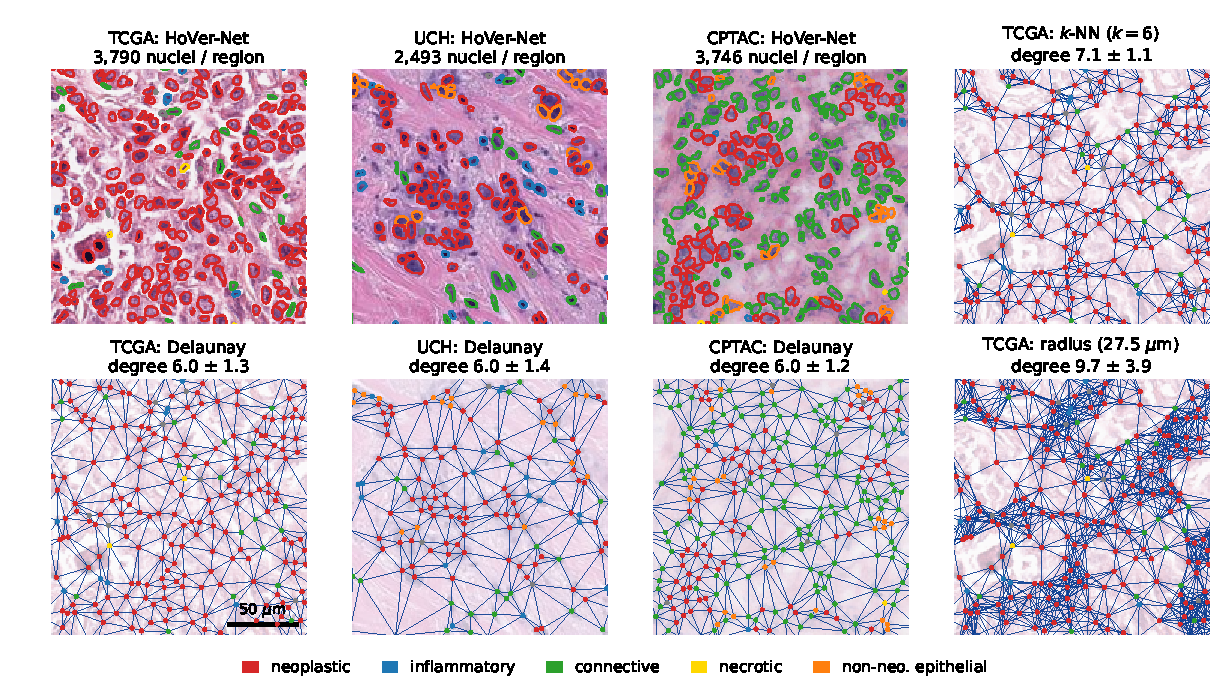
\includegraphics[width=\linewidth]{figures/fig_cohort_graphs.pdf}}
\end{figure}

The node set and the 13 node features are fixed by segmentation; the edge rule is the one
free design choice of the graph branch (\sectionref{sec:related-work}). We rebuild the edges
of every $N=2$ TCGA region with the two rules that compete with Delaunay triangulation,
symmetrised $k$-nearest neighbours ($k=6$) and a fixed radius of $27.5\,\mu$m (110 pixels), and
retrain the graph-only and gated models with all else held fixed (\tableref{tab:edge}).
\figureref{fig:cohort-graphs} shows why the rules behave differently. Delaunay has a mean
degree of 6.0 in all three cohorts although their nucleus counts differ by half (2,493 nuclei
in the UCH region versus 3,790 in TCGA), and $k$-NN is equally density-blind (7.1 $\pm$ 1.1)
but adds chords across empty stroma. The radius graph alone encodes local density, with a mean
degree of 12.1 that ranges from 5 to 22 between regions (5th--95th percentile) and 2.2\% isolated nuclei, and
it therefore changes with the cohort's cellularity and with any residual scale mismatch from
super-resolution.

\begin{table}[htbp]
\floatconts
  {tab:edge}
  {\caption{Edge rule ablation on TCGA at $N=2$ (five-fold AUROC, \%, mean $\pm$ SD). Nodes,
  node features, splits and seeds are identical across rules.}}
  {\small
  \begin{tabular}{llccc}
  \hline
  Target & Model & Delaunay & $k$-NN ($k=6$) & Radius ($27.5\,\mu$m) \\
  \hline
  RS   & Graph & 76.2 $\pm$ 3.5 & EDGE-KNN-ODX-GRAPH & EDGE-RAD-ODX-GRAPH \\
       & Gated & 85.1 $\pm$ 3.9 & EDGE-KNN-ODX-GATED & EDGE-RAD-ODX-GATED \\
  \hline
  PR   & Graph & 65.5 $\pm$ 3.0 & EDGE-KNN-PR-GRAPH & EDGE-RAD-PR-GRAPH \\
       & Gated & 76.8 $\pm$ 3.3 & EDGE-KNN-PR-GATED & EDGE-RAD-PR-GATED \\
  \hline
  HER2 & Graph & 62.1 $\pm$ 3.5 & EDGE-KNN-HER2-GRAPH & EDGE-RAD-HER2-GRAPH \\
       & Gated & 70.3 $\pm$ 4.6 & EDGE-KNN-HER2-GATED & EDGE-RAD-HER2-GATED \\
  \hline
  \end{tabular}}
\end{table}

% TODO: results paragraph for tab:edge once Results/runs/region5fold_edge_{knn6,radius110} finish

\subsection{Where Does the Signal Live?}
\label{sec:where-signal-lives}

To relate the predictions to quantities a pathologist can read, we summarise every $N=2$
region by fourteen descriptors computed directly from the HoVer-Net output and the Delaunay
graph, in physical units: nuclear density and the fraction of each cell type (composition);
the median area, area coefficient of variation (CV), aspect ratio and convexity of the
neoplastic nuclei (nuclear morphology); and the median Delaunay side length, clustering
coefficient, number of nuclei within $30\,\mu$m and the CV of Voronoi cell areas
(architecture). Descriptors are averaged over all regions of a patient and tested
univariately: Spearman's $\rho$ against the continuous RS (RNA-derived in TCGA, clinical in
UCH) and the AUROC of the raw descriptor for PR and HER2 status, with Benjamini--Hochberg
correction within each column (\tableref{tab:morph}).

\begin{table}[htbp]
\floatconts
  {tab:morph}
  {\caption{Patient-level association of region morphology with the targets. $\rho$: Spearman
  correlation with the continuous RS. AUROC: discrimination by the raw descriptor ($<50$: lower in
  positive patients). $^{*}$\,$q<0.05$, $^{**}$\,$q<0.001$ (Benjamini--Hochberg within column).
  TCGA $n$ = 1,038 / 986 / 843 patients; UCH $n$ = 416 / 499. UCH HER2 (9 positives) is omitted.}}
  {\small
  \begin{tabular}{lccc|cc}
  \hline
   & \multicolumn{3}{c|}{TCGA} & \multicolumn{2}{c}{UCH} \\
  Descriptor & RS $\rho$ & PR AUROC & HER2 AUROC & RS $\rho$ & PR AUROC \\
  \hline
  Nuclei per mm$^2$          & $+0.23^{**}$ & $0.44^{*}$  & 0.47        & $+0.03$      & 0.50 \\
  Neoplastic fraction        & $+0.19^{**}$ & $0.45^{*}$  & 0.49        & $+0.08$      & 0.47 \\
  Inflammatory fraction      & $+0.07^{*}$  & $0.45^{*}$  & 0.56        & $+0.01$      & 0.48 \\
  Connective fraction        & $-0.28^{**}$ & $0.60^{**}$ & 0.49        & $-0.11$      & 0.55 \\
  Necrotic fraction          & $+0.21^{**}$ & $0.40^{**}$ & 0.53        & $+0.07$      & 0.51 \\
  Non-neopl.\ epith.\ fraction & $-0.24^{**}$ & $0.58^{**}$ & 0.45      & $-0.10$      & 0.54 \\
  \hline
  Neopl.\ nuclear area       & $+0.03$      & 0.46        & 0.51        & $+0.06$      & 0.51 \\
  Neopl.\ area CV            & $+0.47^{**}$ & $0.33^{**}$ & $0.61^{**}$ & $+0.21^{**}$ & 0.50 \\
  Neopl.\ aspect ratio       & $+0.03$      & 0.51        & 0.53        & $-0.13^{*}$  & 0.49 \\
  Neopl.\ convexity          & $-0.27^{**}$ & 0.54        & 0.46        & $-0.12$      & 0.47 \\
  \hline
  Delaunay side length       & $-0.14^{**}$ & 0.52        & 0.56        & $-0.01$      & 0.50 \\
  Clustering coefficient     & $-0.06^{*}$  & 0.51        & 0.50        & $-0.11$      & 0.51 \\
  Nuclei within 30\,$\mu$m   & $+0.13^{**}$ & 0.48        & 0.43        & $-0.04$      & 0.51 \\
  Voronoi area CV            & $-0.15^{**}$ & $0.57^{**}$ & 0.47        & $-0.11$      & 0.55 \\
  \hline
  \end{tabular}}
\end{table}

One descriptor dominates. The CV of neoplastic nuclear area, a direct measure of nuclear
pleomorphism, correlates with the RS at $\rho=0.47$ in TCGA, is the only descriptor associated
with all three targets (higher in PR$-$ and in HER2+ patients), and is the only one that
replicates on the clinical RS of UCH ($\rho=0.21$, $q<0.001$). Irregular nuclear outlines
(lower convexity), necrosis and a tumour-rich, stroma-poor composition also accompany a high
RS in TCGA, matching the pleomorphism and proliferation components of histological grade
\citep{elston1991} that the RS proliferation group tracks. Median nuclear size, by contrast, is
unrelated to any target, so it is the variability of the nuclei rather than their size that
carries the signal. The compositional associations do not replicate on UCH, whose patients were
referred for the assay and are almost all ER+ and HER2$-$ (97\% and 98\%), so the cohort spans a
narrower biological range than TCGA; no
descriptor separates PR status there, in line with the weak external PR transfer of
\tableref{tab:external}. Because pleomorphism is a property of a population of nuclei, it can be
estimated from a few thousand nuclei, which is what two regions already provide; this offers one
explanation for why the RS saturates at small $N$.

\section{Discussion}
\label{sec:discussion}

% ~1 page

\section{Conclusion}
\label{sec:conclusion}

% ~0.3 pages

\clearpage  % Acknowledgements, references and appendix do not count toward the page limit

% Will not appear in the anonymised version -- MIDL is single-blind, so this is kept.
\midlacknowledgments{}

\bibliography{references}

\appendix

\section{Implementation Details}
\label{app:implementation-details}

\section{Additional Results}
\label{app:additional-results}

\end{document}